\chapter{Experiments and Results}
\label{ch:exp}

\section{Setup}
\paragraph{Data.} The 30 pre-processed worlds in \texttt{data/worlds} (10-minute
windows of one simulated trace, 2959 tasks in total) are split into 20
\emph{training} worlds (0--19) and 10 \emph{test} worlds (20--29). Each world is
truncated to its first 100 tasks; satellites are derived from the server
profiles in the world's CSV, with a fixed per-world seed so that every method
sees exactly the same scenarios.

\paragraph{Training.} During training the world used for fitness evaluation
changes every 10 generations, cycling through the training worlds (a fixed
schedule, unlike the convergence-triggered reset of \texttt{main.py}, so that
runs are comparable). Unless stated otherwise: population 100, maximum depth 4,
hoist rate 0.05, 300 generations, weights $(w_C,w_R,w_E)=(0.60,0.25,0.15)$.
Each configuration is repeated with 10 seeds.

\paragraph{Model selection and testing.} Fitness is normalised across the
population, so it is not comparable between worlds. After training, the 20
fittest individuals are re-scored on all training worlds with the raw
objectives; the one with the highest mean completion ratio (ties: lowest
response time) is kept and evaluated on the test worlds. All numbers below are
means over the test worlds, then mean $\pm$ standard deviation over seeds.

\paragraph{Baselines.} Hand-written priority functions run through the same
decoder: FCFS (score $=-a_j$), shortest job first ($-(e_j+t_j)$), least-loaded
satellite ($-$completed tasks), and most remaining energy. We also report the
average of the \emph{untrained} random trees of generation~0.

\paragraph{Metrics.} Completion ratio $C$, mean response time $R$ (only over
scheduled tasks), and total energy $\mathcal{E}$ (Section~\ref{ch:problem}).
Reproduce with \texttt{thesis/experiments/run\_experiments.py} and
\texttt{make\_report.py}.

\section{Main Comparison}
Table~\ref{tab:main} compares the evolved schedulers (1000 generations, the
other parameters as above) with the baselines.
\begin{table}[h]
\centering\small
\begin{tabular}{lccc}\toprule
Method & Completion ratio $C$ & Mean response $R$ (min) & Energy $\mathcal{E}$\\\midrule
FCFS (first-fit) & 0.204 & 20.60 & 158.7\\
Shortest job first & 0.268 & 16.75 & 159.0\\
Least-loaded satellite & 0.216 & 20.46 & 162.0\\
Most energy left & 0.214 & 20.24 & 157.6\\
Random trees (initial population) & 0.198 $\pm$ 0.003 & 19.29 $\pm$ 0.19 & 159.0 $\pm$ 0.2\\
\midrule
Evolved GP (10 seeds) & 0.197 $\pm$ 0.018 & 13.69 $\pm$ 0.34 & 156.8 $\pm$ 0.2\\\bottomrule
\end{tabular}
\caption{Test-world performance. Higher $C$ is better; lower $R$ and $\mathcal{E}$ are better.}
\label{tab:main}
\end{table}

The evolved rules cut the mean response time to $13.7$\,min, against $16.8$\,min
for the best baseline (SJF) and $19.3$\,min for random trees, with very small
variance across seeds. They do \emph{not} schedule more tasks: with 1000
generations $C=0.197$, no better than random trees and below SJF ($0.268$).
Energy differs by only about 1\% between all methods.

This is a consequence of how the objectives interact. $R$ is averaged over the
tasks that were actually scheduled, so a rule that schedules only a few, short
tasks has a low $R$ and still scores well on the response-time term of the
fitness. Longer training drives the population towards extremely small trees
(mean size 2.4 at 1000 generations) that exploit this. Hence the result should
be read as ``the fitness as currently defined is partly misaligned with the
goal of completing tasks'', and not as evidence that GP cannot beat the
baselines on $C$ (see below, where shorter training and a completion-only
fitness give higher $C$).

\begin{figure}[h]
\centering
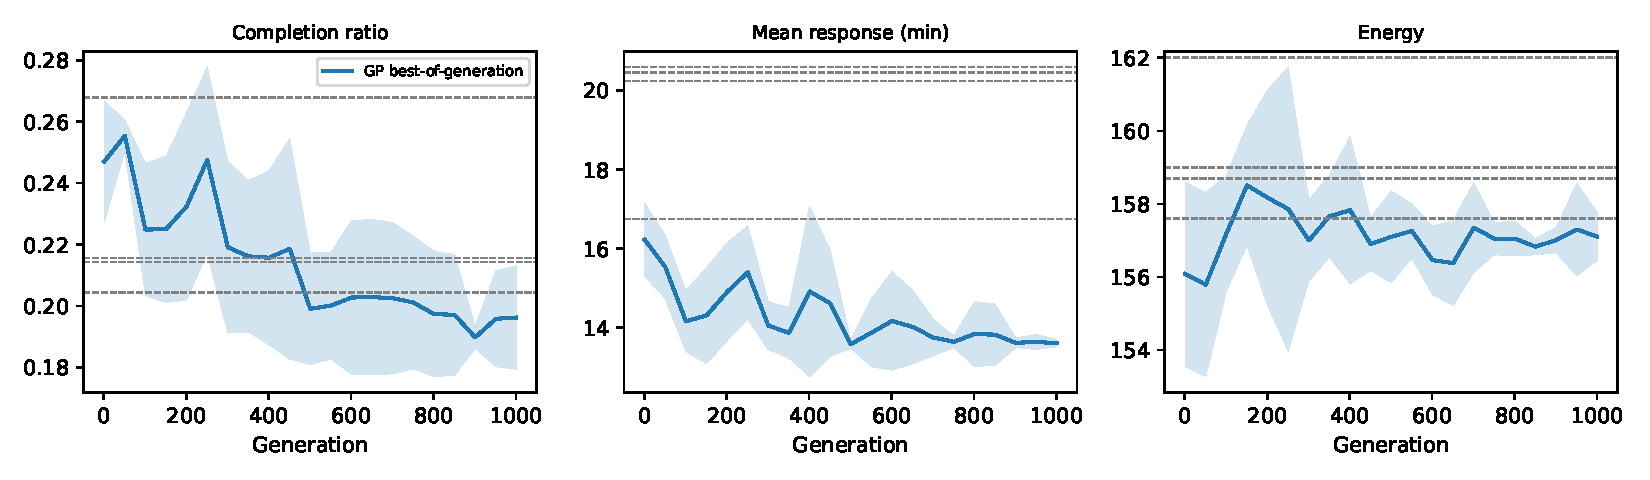
\includegraphics[width=\textwidth]{experiments/results/convergence.pdf}
\caption{Test-world metrics of the best individual of each generation (mean $\pm$
std over 10 seeds). Dashed lines: the four baselines.}
\label{fig:conv}
\end{figure}

Figure~\ref{fig:conv} shows the metrics of the current best individual over
the 1000 generations: $R$ drops from about 16.2 to 14.3\,min within the first 150 generations
(13.6 at the end), while the completion ratio of the best individual goes down
from 0.25 to 0.20.

\section{Parameter Study}
Tables~\ref{tab:depth}--\ref{tab:weights} vary one parameter at a time around
the default configuration (300 generations).

\begin{table}[h]\centering\small\begin{tabular}{lcccc}\toprule
Max.\ depth & $C$ & $R$ (min) & $\mathcal{E}$ & Tree size\\\midrule
2 & 0.202 $\pm$ 0.021 & 13.69 $\pm$ 0.24 & 157.3 $\pm$ 1.2 & 2.0\\
3 & 0.197 $\pm$ 0.019 & 13.64 $\pm$ 0.20 & 156.5 $\pm$ 1.3 & 2.0\\
4 & 0.228 $\pm$ 0.032 & 14.63 $\pm$ 1.16 & 156.1 $\pm$ 1.7 & 7.2\\
5 & 0.222 $\pm$ 0.027 & 13.88 $\pm$ 0.49 & 158.0 $\pm$ 2.0 & 6.2\\
6 & 0.240 $\pm$ 0.019 & 14.51 $\pm$ 0.86 & 157.3 $\pm$ 3.0 & 16.7\\
7 & 0.220 $\pm$ 0.031 & 14.20 $\pm$ 0.85 & 158.7 $\pm$ 2.6 & 11.0\\
\bottomrule
\end{tabular}
\caption{Maximum tree depth.}\label{tab:depth}\end{table}
\begin{table}[h]\centering\small\begin{tabular}{lcccc}\toprule
Population & $C$ & $R$ (min) & $\mathcal{E}$ & Tree size\\\midrule
20 & 0.199 $\pm$ 0.015 & 15.72 $\pm$ 3.42 & 157.8 $\pm$ 1.2 & 1.8\\
50 & 0.212 $\pm$ 0.031 & 14.22 $\pm$ 0.86 & 156.7 $\pm$ 1.4 & 5.8\\
100 & 0.228 $\pm$ 0.032 & 14.63 $\pm$ 1.16 & 156.1 $\pm$ 1.7 & 7.2\\
200 & 0.247 $\pm$ 0.021 & 14.95 $\pm$ 0.88 & 155.7 $\pm$ 2.4 & 12.7\\
400 & 0.250 $\pm$ 0.005 & 14.75 $\pm$ 0.81 & 155.7 $\pm$ 2.8 & 10.6\\
\bottomrule
\end{tabular}
\caption{Population size.}\label{tab:pop}\end{table}
\begin{table}[h]\centering\small\begin{tabular}{lcccc}\toprule
Generations & $C$ & $R$ (min) & $\mathcal{E}$ & Tree size\\\midrule
50 & 0.252 $\pm$ 0.001 & 15.72 $\pm$ 0.37 & 155.6 $\pm$ 0.5 & 13.9\\
100 & 0.241 $\pm$ 0.023 & 14.84 $\pm$ 1.15 & 157.2 $\pm$ 2.7 & 8.8\\
300 & 0.228 $\pm$ 0.032 & 14.63 $\pm$ 1.16 & 156.1 $\pm$ 1.7 & 7.2\\
1000 & 0.197 $\pm$ 0.018 & 13.69 $\pm$ 0.34 & 156.8 $\pm$ 0.2 & 2.4\\
\bottomrule
\end{tabular}
\caption{Number of generations.}\label{tab:gens}\end{table}
\begin{table}[h]\centering\small\begin{tabular}{lcccc}\toprule
Hoist rate & $C$ & $R$ (min) & $\mathcal{E}$ & Tree size\\\midrule
0.0 & 0.232 $\pm$ 0.030 & 14.69 $\pm$ 0.91 & 157.6 $\pm$ 2.9 & 10.9\\
0.05 & 0.228 $\pm$ 0.032 & 14.63 $\pm$ 1.16 & 156.1 $\pm$ 1.7 & 7.2\\
0.2 & 0.196 $\pm$ 0.015 & 13.60 $\pm$ 0.04 & 157.1 $\pm$ 0.5 & 1.2\\
\bottomrule
\end{tabular}
\caption{Hoist rate.}\label{tab:hoist}\end{table}
\begin{table}[h]\centering\small\begin{tabular}{lcccc}\toprule
World switch period (gen.) & $C$ & $R$ (min) & $\mathcal{E}$ & Tree size\\\midrule
1 & 0.208 $\pm$ 0.025 & 13.65 $\pm$ 0.18 & 157.9 $\pm$ 1.4 & 3.5\\
10 & 0.228 $\pm$ 0.032 & 14.63 $\pm$ 1.16 & 156.1 $\pm$ 1.7 & 7.2\\
50 & 0.267 $\pm$ 0.001 & 15.39 $\pm$ 0.72 & 160.8 $\pm$ 3.0 & 15.7\\
$\infty$ & 0.258 $\pm$ 0.007 & 15.81 $\pm$ 0.43 & 157.3 $\pm$ 1.6 & 17.2\\
\bottomrule
\end{tabular}
\caption{Number of generations between world changes ($\infty$: one training world).}\label{tab:switch}\end{table}
\begin{table}[h]\centering\small\begin{tabular}{lcccc}\toprule
Weights $(w_C,w_R,w_E)$ & $C$ & $R$ (min) & $\mathcal{E}$ & Tree size\\\midrule
(0.6, 0.25, 0.15) & 0.228 $\pm$ 0.032 & 14.63 $\pm$ 1.16 & 156.1 $\pm$ 1.7 & 7.2\\
(1.0, 0.0, 0.0) & 0.254 $\pm$ 0.010 & 16.57 $\pm$ 0.65 & 160.3 $\pm$ 2.3 & 13.2\\
(0.34, 0.33, 0.33) & 0.211 $\pm$ 0.041 & 16.87 $\pm$ 1.81 & 156.9 $\pm$ 1.4 & 4.6\\
(0.2, 0.4, 0.4) & 0.203 $\pm$ 0.041 & 17.06 $\pm$ 1.94 & 157.8 $\pm$ 1.0 & 4.2\\
\bottomrule
\end{tabular}
\caption{Fitness weights.}\label{tab:weights}\end{table}

\begin{itemize}
  \item \textbf{Depth} (Table~\ref{tab:depth}). Depths 2--3 give trivial trees
        (size 2) with $C\approx0.20$; depth $\ge4$ gives larger trees and
        $C$ between $0.22$ and $0.24$. Differences between depths 4--7 are within one standard deviation.
  \item \textbf{Population} (Table~\ref{tab:pop}). $C$ grows with population size
        ($0.199$ at 20 to $0.250$ at 400), the clearest monotone trend, with lower
        variance for large populations.
  \item \textbf{Generations} (Table~\ref{tab:gens}). Contrary to expectation, $C$
        \emph{falls} with more generations ($0.252$ at 50, $0.197$ at 1000) while $R$
        falls too, which is the misalignment discussed above.
  \item \textbf{Hoist rate} (Table~\ref{tab:hoist}). 0 and 0.05 are equivalent; 0.2
        collapses the trees to a single node (size 1.2) and loses completion ratio.
  \item \textbf{World switching} (Table~\ref{tab:switch}). Changing the world every
        generation hurts ($C=0.208$); slower switching (50 generations) or a single
        world gives the highest $C$ ($0.267$, $0.258$) but a higher $R$ and larger
        trees. On this dataset we found no sign that a single training world overfits
        more than cycling through worlds.
  \item \textbf{Fitness weights} (Table~\ref{tab:weights}). Weighting completion only
        gives the best $C$ ($0.254$) at the price of a longer $R$ ($16.6$\,min); giving
        more weight to $R$ and $\mathcal{E}$ lowers $C$ to about $0.20$ and does not
        lower $R$.
\end{itemize}

\section{Evolved Rules}
Table~\ref{tab:trees} lists the three best rules of the main runs by test completion ratio.
\begin{table}[h]\centering\small
\begin{enumerate}
\item $C=0.248$, size 15:\\
{\small\texttt{((job.arrivalTime - job.executionTime) - ((MAX(job.disk, job.arrivalTime) * MAX(sat.completedTasks, job.executionTime)) /? MAX(sat.networkBusyUntil, sat.bandwidth)))}}
\item $C=0.191$, size 1:\\
{\small\texttt{job.arrivalTime}}
\item $C=0.191$, size 1:\\
{\small\texttt{job.arrivalTime}}
\end{enumerate}
\caption{Best evolved rules (\texttt{/?} is protected division).}\label{tab:trees}
\end{table}
Many evolved rules reduce to a single terminal, \texttt{job.arrivalTime}, i.e.\
an FCFS-like ordering with the decoder's first-fit satellite choice; the larger
rules combine task execution time and arrival time (a shortest-job-like term)
with satellite load and bandwidth.

\section{Threats to Validity}
\begin{itemize}
  \item One trace, split into consecutive windows: train and test worlds come from the same
        distribution and test worlds are temporally adjacent to training ones.
  \item Worlds are limited to 100 tasks and completion ratios are low
        ($\approx0.2$--$0.3$) because the operational window and energy constraints of the
        decoder reject most pairs; conclusions may change with other loads.
  \item Mean response time over scheduled tasks only (see above); $\mathcal{E}$ varies very little between methods.
  \item The difference between many configurations is of the order of one standard deviation over 10 seeds;
        no significance test was run.
  \item Models are selected with a heuristic (training completion ratio) rather than the fitness itself.
  \item All results use the default selection rule~\eqref{eq:sel-index}. Task-only rules, including
        the FCFS and shortest-job-first baselines and the many evolved single-terminal rules, therefore
        take the first feasible satellite. The earliest-free rule of Section~\ref{sec:ties} has not been
        evaluated (configurations \texttt{tiebreak*} of \texttt{run\_ablation.py}); it changes the
        decoder, so the baselines must be re-scored with it as well.
  \item All results use the population-relative fitness. The fixed-bound fitness of
        Section~\ref{sec:fixed}, designed to remove the misalignment discussed above, has not
        been evaluated yet (configurations \texttt{fixed} and \texttt{fixed+clones+worlds3} of
        \texttt{run\_ablation.py}).
\end{itemize}
